\begin{figure}
\centering
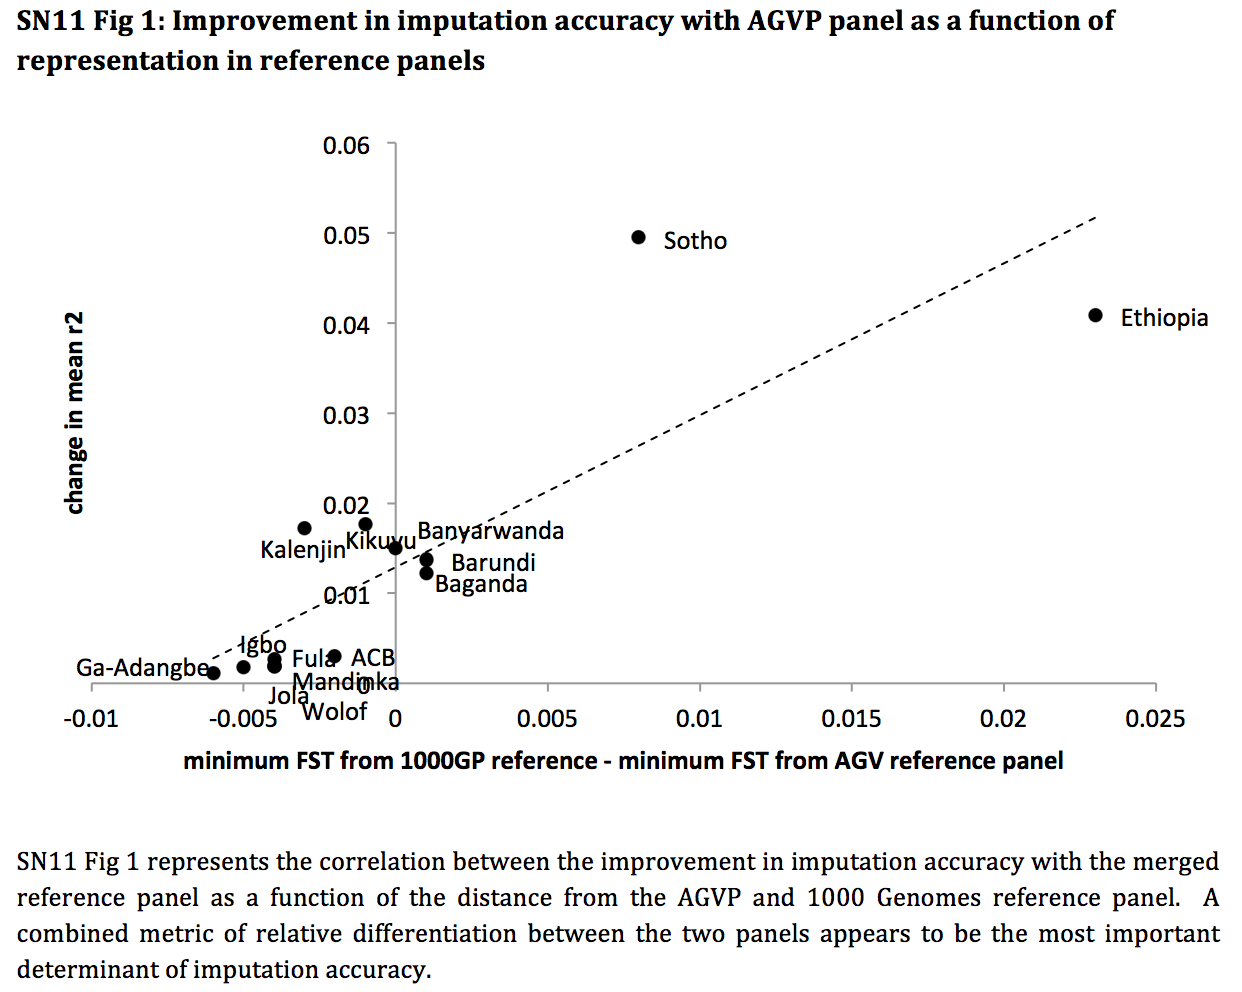
\includegraphics[trim={0 3.5cm 0cm 1.25cm},clip,width=0.75\textwidth]{fig/SN11f1}
\caption[
Improvement in imputation accuracy for each population using two different reference panels as a function of difference in minimum \glssymbol{FST} between each population in either of the two reference panels.]{
Correlation between improvement in imputation accuracy (y-axis) and smallest \glssymbol{FST} from a \gls{1000G} population (x-axis). The \glssymbol{FST} is calculated between each African population and each of the \gls{1000G} populations. The smallest value is plotted on the x-axis. The improvement in imputation accuracy - as measured by change in overall \glssymbol{r2} reported by IMPUTE2 when using a \gls{1000G} and \gls{1000G}+\gls{AGV} reference panel - is plotted on the y-axis. Presumably Sotho improves more than any other population, because no South African population is present in \gls{1000G}, whereas the \gls{AGV} reference panel contains a Zulu population. Likewise an infinitesimal improvement is observed for the Igbo population, because the neighboring Yoruba population is already present in \gls{1000G}. \glssymbol{FST} values calculated by Deepti Gurdasani and Savita Karthikeyan.
%Correlation between the improvement in imputation accuracy with the merged reference panel as a function of the difference in minimum \glssymbol{FST} relative to populations constituting the \gls{1000G} reference panel and the merged reference panel. \glssymbol{FST} values calculated by Deepti Gurdasani and Savita Karthikeyan.
}
\label{fig:SN11f1}
\end{figure}